\LevelOneTitle{粘性流动基础}

\LevelTwoTitle{粘性流体一点应力状态}

对于理想流体,一点应力$p = p(x, y, z)$,方向垂直于作用面并指向流体内部,大小与作用面方位无关,只是作用点位置的函数。

对于粘性流体则不然,其一点应力分为法向应力$\sigma_n$和切向应力$\tau_n$,大小与作用面有关。

\LevelTwoTitle{*N-S方程}

\LevelThreeTitle{本构方程}

本构方程反映应力与变形率的关系。

\LevelThreeTitle{N-S方程}

N-S方程是牛顿第二定律应用于流体微团,物理意义是流体微团所受重力和表面力的合力等于流体微团质量乘加速度。

可以了解不可压流体的N-S方程的形式:

\begin{equation}
	\dfrac{\mathrm{D} \vec{V}}{\mathrm{D} t} = \vec{g} - \dfrac{1}{\rho} \nabla p + \nu \nabla^2 \vec{V}
\end{equation}

若是理想流体,则去掉粘性项,就成为欧拉方程(式\ref{eq4.2}),即

\begin{equation*}
	\dfrac{\mathrm{D} \vec{V}}{\mathrm{D} t} = \vec{g} - \dfrac{1}{\rho} \nabla p
\end{equation*}

若流体静止,则加速度为0,就成为静止流体平衡微分方程(式\ref{eq2.1})的形式,即

\begin{equation*}
	0 = \vec{g} - \dfrac{1}{\rho} \nabla p
\end{equation*}

\LevelTwoTitle{流动状态}

\LevelThreeTitle{不同流态的特点}

流体流态分为:层流、转捩和湍流。

\begin{enumerate}
	\item 层流,分层流动,质点轨迹光滑,流动稳定;
	\item 转捩,层与层之间开始掺混;
	\item 湍流,层与层之间剧烈掺混,质点轨迹杂乱无章,流体做复杂无规则的随机运动,属于三维非定常有旋运动。
\end{enumerate}

\LevelThreeTitle{雷诺数}

雷诺数$Re$是决定流态的判据,物理意义是惯性力和粘性力之比,数学表达式为

\begin{equation}
	Re = \dfrac{\rho V L}{\mu} = \dfrac{V L}{\nu}
\end{equation}

其中,$V$是特征速度,$L$是特征长度。

\begin{table}[H]
	\centering
	\begin{tabular}{ccc}
		\toprule[1pt]
		流动问题 & 特征速度 & 特征长度 \\
		\hline
		圆管内流 & 管内流速$V$ & 圆管内径$D$ \\
		平板边界层 & 无穷来流速度$U_{\infty}$ & 距前缘距离$x$或边界层厚度$\delta$\\
		\bottomrule[1pt]
	\end{tabular}
    \caption{不同流动问题有不同的特征物理量}
\end{table}

雷诺数$Re$判断流态的原理(容易考简答题):

\begin{enumerate}
	\item $Re$较小时,粘性力影响显著,扰动受粘性阻尼作用衰减,此时为层流;
	\item $Re$较大时,惯性力影响显著,惯性力对扰动的放大作用远超粘性阻尼作用,此时为湍流。
\end{enumerate}

\LevelTwoTitle{三种解析解}

可以不掌握具体表达式,但要知道速度和切应力分布的图形以及最大速度和平均速度的关系。

\begin{enumerate}
	\item 平面泊肃叶流动,$u_{\text{max}} = 1.5 \overline{V}$。
	\begin{figure}[H]
		\centering
		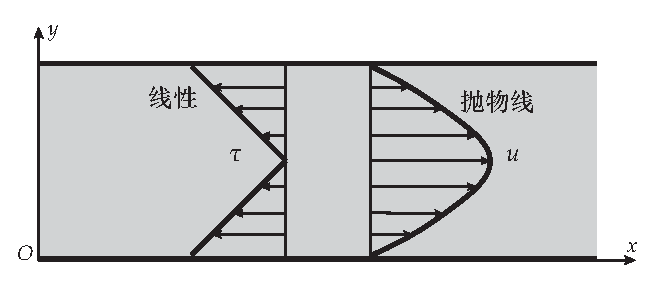
\includegraphics[scale=0.6]{figures/平面泊肃叶.eps}
		\caption{平面泊肃叶流动的速度和切应力分布}
	\end{figure}
	\item 平面库埃特-泊肃叶流动,斜直线:$\displaystyle \pdv{p}{x} = 0$;斜直线右侧(斜直线+抛物线,顺压梯度):$\displaystyle \pdv{p}{x} < 0$;斜直线左侧(斜直线$-$抛物线,逆压梯度):$\displaystyle \pdv{p}{x} > 0$。
	\begin{figure}[H]
		\centering
		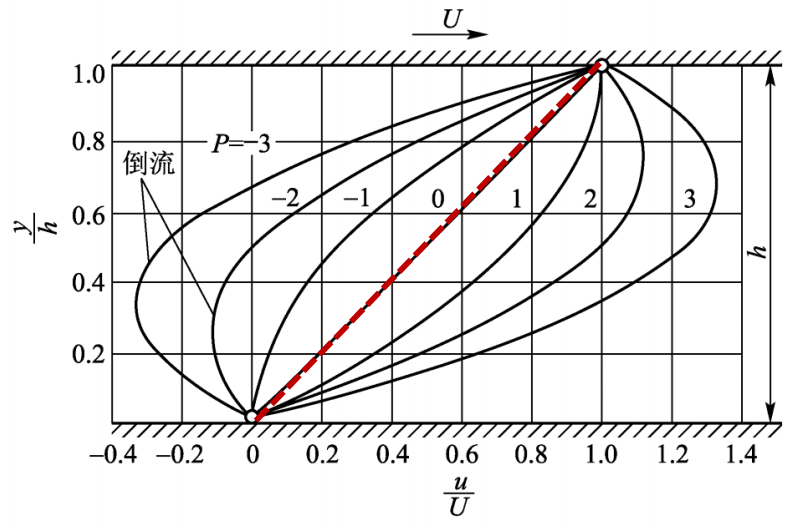
\includegraphics[scale=0.35]{figures/平面库埃特.png}
		\caption{平面库埃特-泊肃叶流动的速度分布}
	\end{figure}
	\item 圆管内泊肃叶流动,$V_{z_{\text{max}}} = 2 \overline{V}_z$。
	\begin{figure}[H]
		\centering
		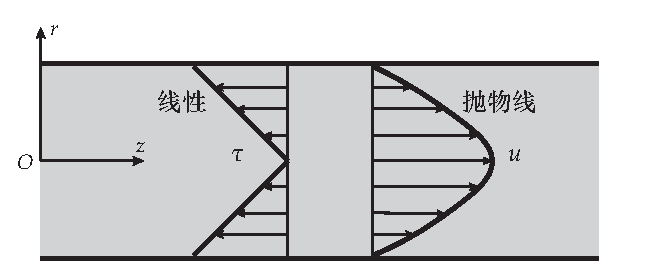
\includegraphics[scale=0.6]{figures/圆管泊肃叶.eps}
		\caption{圆管内泊肃叶流动的速度和切应力分布}
	\end{figure}
\end{enumerate}

\LevelTwoTitle{湍流物理量}

\begin{enumerate}
	\item 瞬时物理量$\eta$;
	\item 时均物理量$\displaystyle \overline{\eta} = \dfrac{1}{T} \int_{t_0}^{t_0 + T} \eta(t) \dd{t}$;
	\item 脉动物理量$\eta' = \eta - \overline{\eta}$。
\end{enumerate}

脉动物理量的时均值(2021·选择)

\begin{equation}
	\overline{\eta'} = \overline{\eta - \overline{\eta}} = \overline{\eta} - \overline{\eta} = 0
\end{equation}

\LevelTwoTitle{*雷诺应力}

\begin{enumerate}
	\item 层流切应力
	\begin{equation*}
		\tau = \mu\dv{u}{y}
	\end{equation*}
    \item 湍流切应力
    \begin{equation}
    	\tau = \mu\dv{u}{y} - \rho \overline{u' v'}
    \end{equation}
\end{enumerate}

其中,$\rho \overline{u' v'}$就是雷诺应力,由流体微团脉动导致动量横向传递引起,是流体微团在$x$方向上动量的时均值。

对于圆管湍流,在层流底层中,分子粘性应力$\displaystyle \mu \dv{u}{y}$占主导地位;在湍流核心区,雷诺应力$\rho \overline{u' v'}$占主导地位。

\LevelTwoTitle{圆管湍流}

只需要定性了解不同区域速度分布的情况,不必掌握表达式。

\begin{enumerate}
	\item 近壁区层流底层,速度为线性分布;
	\item 湍流核心区,速度为对数分布或幂律分布,随着流速的增加,幂律分布中的$n$也增大,速度分布变得均匀。
\end{enumerate}
